\documentclass[a4paper,12pt]{article}
\usepackage{graphicx} %package to manage images
\graphicspath{ {./figures/} }

%
%% PACKAGE IMPORTS
%%  If any package needed, import it here
%

\usepackage{styles/ibu-thesis}
\usepackage{subcaption}

%
%% MACROS
%%  If any macro needed, define it here
%
\newcommand{\writecommand}[2]{
    \begin{center}
        \texttt{\textbackslash #1\{\##2\#\}} \\
    \end{center}
}


%
%% THESIS TITLE
%
\thesistitle{Title: NFT MARKETPLACE PROJECT for Thesis}

%
%% AUTHOR INFORMATION 
%%  If there is more than 3 author it can be added to list
%%  e.g. \authors[4]{Name of author} and \authorsid[4]{ID of author} etc.
%
\authors[1]{AHMAD YOUSSEF}
\authorsid[1]{117200027}
\authors[2]{Sadiq Tijjani}
\authorsid[2]{119200113}
\authors[3]{Baris Tonbul}
\authorsid[3]{117200054}

%
%% SUPERVISOR INFORMATION
%%  If there is more than 2 supervisor it can be added to list
%%  e.g. \supervisors[3]{Name of supervisor} etc.
%
\supervisors[1]{Dr. Hakan Ayral}

%
%% AFFILIATION INFORMATION
%%  Below information are must
%
\faculty{Faculty of Engineering and Natural Sciences}
\degree{Bachelor of Science}
\department{Department of Computer Engineering}
\submissiondate{Jan, 2022}

%
%% ABSTRACT
%%  In case of more than one paragraph abstracts, use \\ separator only 
%%  to open a new paragraph
%%  e.g. ... paragraph ended here. \\ New paragraph starts here ...
%
\abstract{This project concerns building a digital marketplace that will serve as a meeting point for buyers and sellers of NFTs to come together and trade, the Marketplace will display a gallery of collectibles with their respective prices and bidding details, similar to everyday art auctions. We will be trying to facilitate an easy exchange of value-able assets on the ethereum network.\\
The idea is for any user to use their crypto-wallets to log-in to our website and then be able to easily Mint an NFT for sale or bid for an NFT in the marketplace gallery. Since the NFT has recently gotten alot of attention as more and more people realize the value of it, this has led to a boom in the NFT market and has shown glimpses of a future paradigm shift in the art world.\\
The following report will expand about the topics of blockchain and how it works, the NFT, what it is and how it is connected to blockchain, later in the report we get into the nitty-gritty of how we intend to build our marketplace and then finally in the latter part of the report we illustrate the goal and results expected for the project.}



\begin{document}

%
%% PRELIMINARIES 
%
\maketitle

\addcontentsline{toc}{section}{\abstractname}
\makeabstract

\addcontentsline{toc}{section}{\contentsname}
\maketableofcontents

\addcontentsline{toc}{section}{\listoffigures}
\makelistoffigures



%
%% LIST OF SYMBOLS AND ABBREVIATIONS
%%  Add or remove the symbols and abbreviations that are 
%%  used in your thesis here 
%% List of abbreviations
\addcontentsline{toc}{section}{\listofabbrv}
\makelistofabbrv
\begin{abbrv}
    \item[i.e.] Id est (Latin: this means)
    \item[e.g.] Exempli gratia (Latin: for example)
\end{abbrv}
\newpage

\pagenumbering{arabic} % Do not change
\setcounter{page}{1} % Do not change


%
%% SECTIONS
%%  The thesis starts here
%

\section{INTRODUCTION}



The emergence of blockchain has allowed for recording transactions and tracking assets in any given network, the efficiency, security and transparency this blockchain ledger provides has given opportunities for applications in many areas in human life, most especially in the area of digital legal tender(digital money) as seen in the ever-growing crypto-currency boom. So what exactly is blockchain and how does it work?\\

Blockchain is a peer-to-peer immutable decentralised distributed ledger that allows for recording digital assets transparently without involving any third party intermediary. A decentralized network has a number of advantages over a centralized network including an increase in reliability, transparency and security, Moreover decentralized networks are much less difficult to scale and thus allow for better shared communication and distributed processing. \\

Using this technology, participants can confirm transactions without a need for a central clearing authority. A transaction in the block requires a wallet, a blockchain wallet is a program(or application) that allows users to hold and spend crypto-currencies like Ethereum(ETH) or Bitcoin(BTC), these wallets are secured using crytographic methods(public and private key). The user's private key allows for the user to spend the associated crypto-currencies, in addition, there is also a public key and there is a cryptographic link between the public key and the private key, theoretically, a user can create billions of public key addresses from his/her private key ,once a user creates a public key address, that address is publicly available to all users in the network as an address where they can send crypto-currencies like Bitcoin. Therefore a transaction works thusly;- If User A want to invoke a transaction with User B , A will specify transaction amount and the public key of B, this message is then signed using A's private key, the signed message is the encrypted using a secure hash algorithm(SHA-256), after these steps a block in the ledger will be created representing that transaction is created,  once the block has been created the transaction is then broadcasted over the peer-to-peer network where User B will be listening, User B will then receive and decrypt the message using his/her private key, a concensus algorithm called Proof of work will then use cryptographic proofs to check if the public-private keys pairs are valid, once a transaction is verified, it is combined with other blocks to create a new block of data for the ledger. \\

The blockchain immutable ledger gives way for a number of applications not only in more traditional industrial sectors like healthcare, insurance and other financial services but also into the ownership of digital media assets and collectibles. This is where the Non-fungible token comes into play, the non-fungible token is a class of token that draws it's value from it's uniqueness, NFTs are usually associated with digital art or images with the license to use these assets for a specific reason. The NFT is a unit of data stored on the blockchain ledger that works like a crytographic token, but unlike other such tokens like Bitcoin, Ethereum and XRP, NFTs are not mutually interchangeable hence the name non-fungible tokens. NFTs are created when the blockchains merge together records(blocks) of cryptographic hash with other previously existing blocks creating a data chain of identifiable blocks. The blockchain transaction process ensures authentication of each digital media file by providing a digital signature that is used to track Non-Fungible Token ownership. The NFT has become very popular recently as artists, content creators and the general public realize the value in electronically owning a piece of art and/or other rare collectible items(for example, Jack Dorsey’s first tweet on twitter was sold for 2.9  million dollars as an NFT), one can own a digital media asset as an NFT with the help of an immutable ledger which means that the NFT boom really is a move from the analog traditional way of art collection and ownership to a digital paradigm for art collection and ownership, but just like one can go to the louvre and take a picture of the mona lisa(or re-create it entirely), it is also possible for someone to take the screenshot(digital copy) of an NFT, simply because the ownership of an NFT does not inherently grant intellectual property rights of the asset to the owner. The hope of NFTs is that as we move further and further into the digital age and as the blockchain ledger increasingly finds more and more use in everyday human life(like in voting systems, healthcare systems and social media applications), one can not only own a media asset digitally,  but one can also own the rights and intellectual property to that media asset as well. \\

The main purpose of this project is to build a digital marketplace that allows sellers who are interested in selling their NFTs and buyers who are interested in buying said NFTs to meet and trade. 


\section{Design}
Our website will be a Decentralized application(Dapp), a Dapp is basically an application built on a decentralized network that combines a smart contract and a frontend user interface, Dapps are like other normal web applications except that they run on a peer-to-peer network, such as blockchain. Dapps are very beneficial in that they are resistant to censorship, they are open source and they are blockchain based(built on smart-contracts). Dapps work essentially according to the various logics of the algorithms contained in the smart contracts upon which they are built, smart contracts remove the need for a third party to handle transactions between peers. Since the middle man is replaced by code, all kinds of costs are reduced, including time and money.
To design our Website, we will be using the following design tools:-

\subsection{Next.js}
To develop websites easily, Next.js is to be used since it is a JavaScript framework that enables you to build superfast and extremely user-friendly static websites, as well as web applications using React. In fact, thanks to Automatic Static Optimization, “static” and “dynamic” become one now.
This feature allows Next.js to build hybrid applications that contain both server-rendered and statically generated websites.


\subsection{NPM}

Npm will make it simple for us to share and reuse code or even update it since it is a package manager for Node platform, and if a package references to another package with a git URL, npm depends on a pre-installed git.


\subsection{Solidity}

Solidity is an object-oriented programming language, meaning that it is organized by data or objects rather than functions or logic. Its main purpose is for developing smart contracts for the Ethereum blockchain. A smart contract is a program(collection of functions and states) that runs on the ethereum blockchain, they're not controlled by a user, instead they are deployed to the network and run as programmed. User accounts can then interact with a smart contract by submitting transactions that execute a function defined on the smart contract. Smart contracts for minting token usually implement the ERC 721 standard which defines a minimum interface a smart contract must implement to allow unique tokens to be managed, owned, and traded.
\begin{figure}[h]
\centering
\includegraphics[width=\textwidth]{Screenshot (190)}
\caption{Snapshot Of Implementation of ERC 721 Standard In Solidity}
\end{figure}
\newpage
\subsection{HTML5}

Hypertext Markup Language revision 5 (HTML5) is a markup language for the structure and presentation of World Wide Web contents. HTML5 supports the traditional HTML and XHTML-style syntax and other new features in its markup, New APIs, XHTML and error handling.

\subsection{Hard Hat}

Hardhat is a development environment that helps us to compile, deploy, test, and debug  Ethereum software. It helps developers manage and automate the recurring tasks that are inherent to the process of building smart contracts and dApps, as well as easily introducing more functionality around this workflow.



\subsection{Tailwind CSS}
Tailwind CSS is basically a utility-first CSS framework for rapidly building custom user interfaces. It is a highly customizable, low-level CSS framework that gives you all of the building blocks you need to build bespoke designs without any annoying opinionated styles you have to fight to override.

\subsection{IPFS}
IPFS is a file sharing system that can be leveraged to more efficiently store and share large files. It relies on cryptographic hashes that can easily be stored on a blockchain. Nonetheless, IPFS does not permit users to share files with selected parties. This is necessary, if sensitive or personal data needs to be shared.

IPFS services can be gotten from a number of outlets including Infura and/or Moralis.

\subsection{MetaMask}


MetaMask allows users to store and manage account keys, broadcast transactions, send and receive Ethereum-based cryptocurrencies and tokens, and securely connect to decentralized applications through a compatible web browser or the mobile app's built-in browser.

\subsection{Polygon}

Polygon Matic or Polygon is a framework for developing inter-operable blockchain networks. The framework primarily focuses on addressing some of the prominent setbacks associated with Ethereum. Polygon is able to leverage a new sidechain solution for addressing setbacks such as lack of community governance, throughput complications, transaction speed and poor user experience.The Polygon Ethereum layer 2 scaling solution will help us to facilitate and verify transactions in the marketplace. 




\section{Website Overview}
In the simplest terms, our marketplace(or any Dapp for that matter) is giving the user a way interact with the smart contracts on the blockchain. Basically, our website serves as a front-end user interface through which any user can interact with the back-end(i.e the smart contracts running on the ethereum network) by opting to sell an NFT, buy an NFT, list an NFT etc. Below is an explanaition of the core rudimentary features \footnote{Keep in mind that these features are only preliminary ideas and are very likely to change as we develop the project more.} of our website:-
\subsection{Main Marketplace}
This will be a gallery through which any incoming user can view the digital art on sale and select which he would like to bid for.
\subsection{Mint Tokens}
This will be a button at the top of the marketplace that when clicked, will lead the user to page where he/she is prompted to pick the NFT he/she wants to mint, give it a name, description and price, then mint it for sale. 
\subsection{My NFTs}
This will be a button beside the "Mint Tokens" button that when clicked, will lead the user(if the user has registered his crypto wallet with the website and has purchased  NFTs) to a page that is a gallery of all the NFTs he/she owns.
\subsection{Account Overview}
This will be a button that when clicked will load up the user's account details i.e Gallery of NFTs sold, number of NFTs sold, gross total earnings etc.


\section{Problems encountered}
\begin{itemize}
\item It was difficult to find core rudimentary references or documentation on how to setup, execute and verify(test) a decentralized web application
\item While setting up hard hat we ran into a problem where hard hat wouldn't start up but we were able to fix this issue by migrating our files into a new folder.
\item Some of the  costs were unexpected such as having to pay to increase our data storage on infura.
\item We encountered a problem when we were implementing the login section of our project regarding the backend database(usually called servers) services, the problem being that we don't know yet how using services like moralis or firebase will affect the other parts of the project in the future, for example,if we use a moralis server, we may have to manually connect the moralis server through a separate cloud server and then to our polygon network in order for the project to execute.

\end{itemize}
\begin{figure}[h]
\centering
\includegraphics[width=\textwidth]{Screenshot (189)}
\caption{Screenshot Of Unexpected Error}
\end{figure}

\newpage


\section{Methodology}
Agile methodology is the best methodology for our project as it continues as a cycle:
\begin{figure}[h]
\centering
\includegraphics[width=\textwidth]{agile}
\caption{Agile Methodology}
\end{figure}
\vspace{1cm}
When comparing the agile methodology to other methods, agile method has (39 per-cent success rate, 52 per-cent challenge rate and only 9 per-cent failure rate).The agile methodology allows for continuous production cycles, small collaborative teams(as is ours) and most importantly for us, it is adaptive to change.The processes of plan-design-develop-test provide a straightforward, yet also flexible path way for the completion of this project.

As is encouraged in the agile methodology, at each iteration of working on our project, we will start with defining the initial requirements(timelines,errors to be corrected, features to be added,removed or updated), then we plan the delivery method and design strategy according to the set  expectations. After that, we start working on the project accordingly, we are still in the phase of designing the smart contracts and we will be developing more(of the contracts and of other parts of the project) with the coming semester to release it to the jury.


\section{Previous Works About Project}
The NFT market is still new and and is still in it's infancy but there are a few notable projects that have made a strong impression on the NFT community:-

\subsection{OpenSea}
OpenSea,founded in 2017, is an online decentralized marketplace for NFTs, it is based on the Ethereum ERC-721 standard and Polygon . In August of 2021,  OpenSea recorded well over 3.5 billion dollars in NFT trading volume, rising from about 25 million in 2020. 
\begin{figure}[h]
\centering
\includegraphics[width=\textwidth]{Opensea}
\caption{OpenSea Marketplace}
\end{figure}
%----------------------------------------------------------------------------

\vspace{1cm}

%----------------------------------------------------------------------------

\subsection{Rarible}
Rarible, launched in early 2020, is a platform for creating, buying and trading digital collectibles(otherwise known as NFTs), one of Rarible’s key features is the ability to give previews of content in the forms of previews, trailers, or snippets while locking away the full content for a buyer.
\begin{figure}[h]
\centering
\includegraphics[width=\textwidth]{Rarible}
\caption{Rarible Marketplace}
\end{figure}
%----------------------------------------------------------------------------

\vspace{1cm}

%----------------------------------------------------------------------------

\section{RISK ANALYSIS}
Firstly, there is always the risk of project personnel getting ill with covid and/or other diseases, we believe we have mitigated this by adopting the agile methodology since the methodology is easily adapted to change, so if a member is not able to do a task, another team-member can easily compensate for the loss.\\
There is also a risk of poor time-management, as all group members are in their 4th year of the programs and are doing other side projects and going to work, so it is important to follow the timeline as closely as we can with the help of the agile methodology.\\
There is a risk of our marketplace not getting enough publicity as a result of poor marketing strategies, so it is important to remedy this with very aggressive advertisement.\\
Finally, there is a risk of Unforeseen blocks in the road, meaning that the area of NFT marketplace development is still in it's infancy and therefore is always changing and growing, so as we develop the project more and more into the second semester, we may find that some documentation we may want for new features to add or some servers/websites we want to use may not be available to us as they may be behind a pay wall or not readily found through research.

\section{COSTS}
\begin{itemize}
  \item Infura Developer Package will cost us 50 dollars per month.
  \item Online Courses for basic knowledge and research will cost us about 12 dollars per course.
  \item A secondary drive for storing important files will cost us 15 dollars.
  \item The server hosting service pricing is at yet undefined but will be made clearer as we enquire more into the next semester.
  \item There may be unexpected expenses that manifest themselves as we move into the next semester(having to fix a broken laptop, having to pay for an upgrade to a service etc.)
  \item There is also a marketing and advertisement cost for getting publicity on our marketplace, cost of ads vary with the platforms but we will budget 350 dollars for this.
  \item Finally there is always an implicit opportunity cost of doing any project, any of the group members could be working on or learning something else instead.
\end{itemize}

\section{Timeline}
We plan to execute our project in roughly the fashion that is depicted below:-
\begin{figure}[h]
\centering
\includegraphics[width=\textwidth]{Picture2}
\caption{Project Timeline}
\end{figure}
%----------------------------------------------------------------------------

\vspace{4cm}

%----------------------------------------------------------------------------
\section{Experimental setup}
The experimental setup of our project is as follows:-
\begin{itemize}
    \item Deploying smart contracts involves getting a smart contract address and an application binary interface(ABI) from the source solidity files being deployed into an ethereum network.
    \item Hardhat compilation involves compiling the solidity source code and getting the ABI of the smart contract.
    \item Then on to the hardhat migration which involves deploying the compiled the byte-code of the smart contract to the ethereum network via the hardhat RPC(Remote Procedural Call) provider. An RPC server is an interface provided by an application or service that allows remote clients to connect, pass commands and transfer data. Migrations are JavaScript files that aid in deploying contracts to the Ethereum network. Smart contracts can also be deployed without a migration, the use of migration varies with the development environment and particular features the developer wants for the project.
    \item The hardhat node will then set up an ethereum network node, after running the npx hardhat node command, a local networks is created with 19 accounts generated with pre-loaded ether balance for the local network. After the contracts are deployed, tested and verified the project is then deployed the polygon through a configuration in the hardhat configuration folder and metamask. Polygon will then facilitate and validate the transactions over a testnet, this however will be done after the aforementioned tests validate the contracts contain no errors.
    \item The web3 js is a collection of libraries which allow you to interact with a local ethereum node, using a HTTP or IPC connection. It aids in the interaction between contracts and the user using the UI. The hardhat contract is a better ethereum contract construct for the node and the browser, it helps to directly call a smart contract method in a similar way to calling any java or JS object method instead of sending raw transactions over network, a developer doesn't have to use this method, the processes work the same with or without it, just a better way to call contract methods.
    \item Finally the User UI with metamask extension serve as a way for the user to invoke transaction on the blockchain.
\end{itemize}
\begin{figure}[h]
\centering
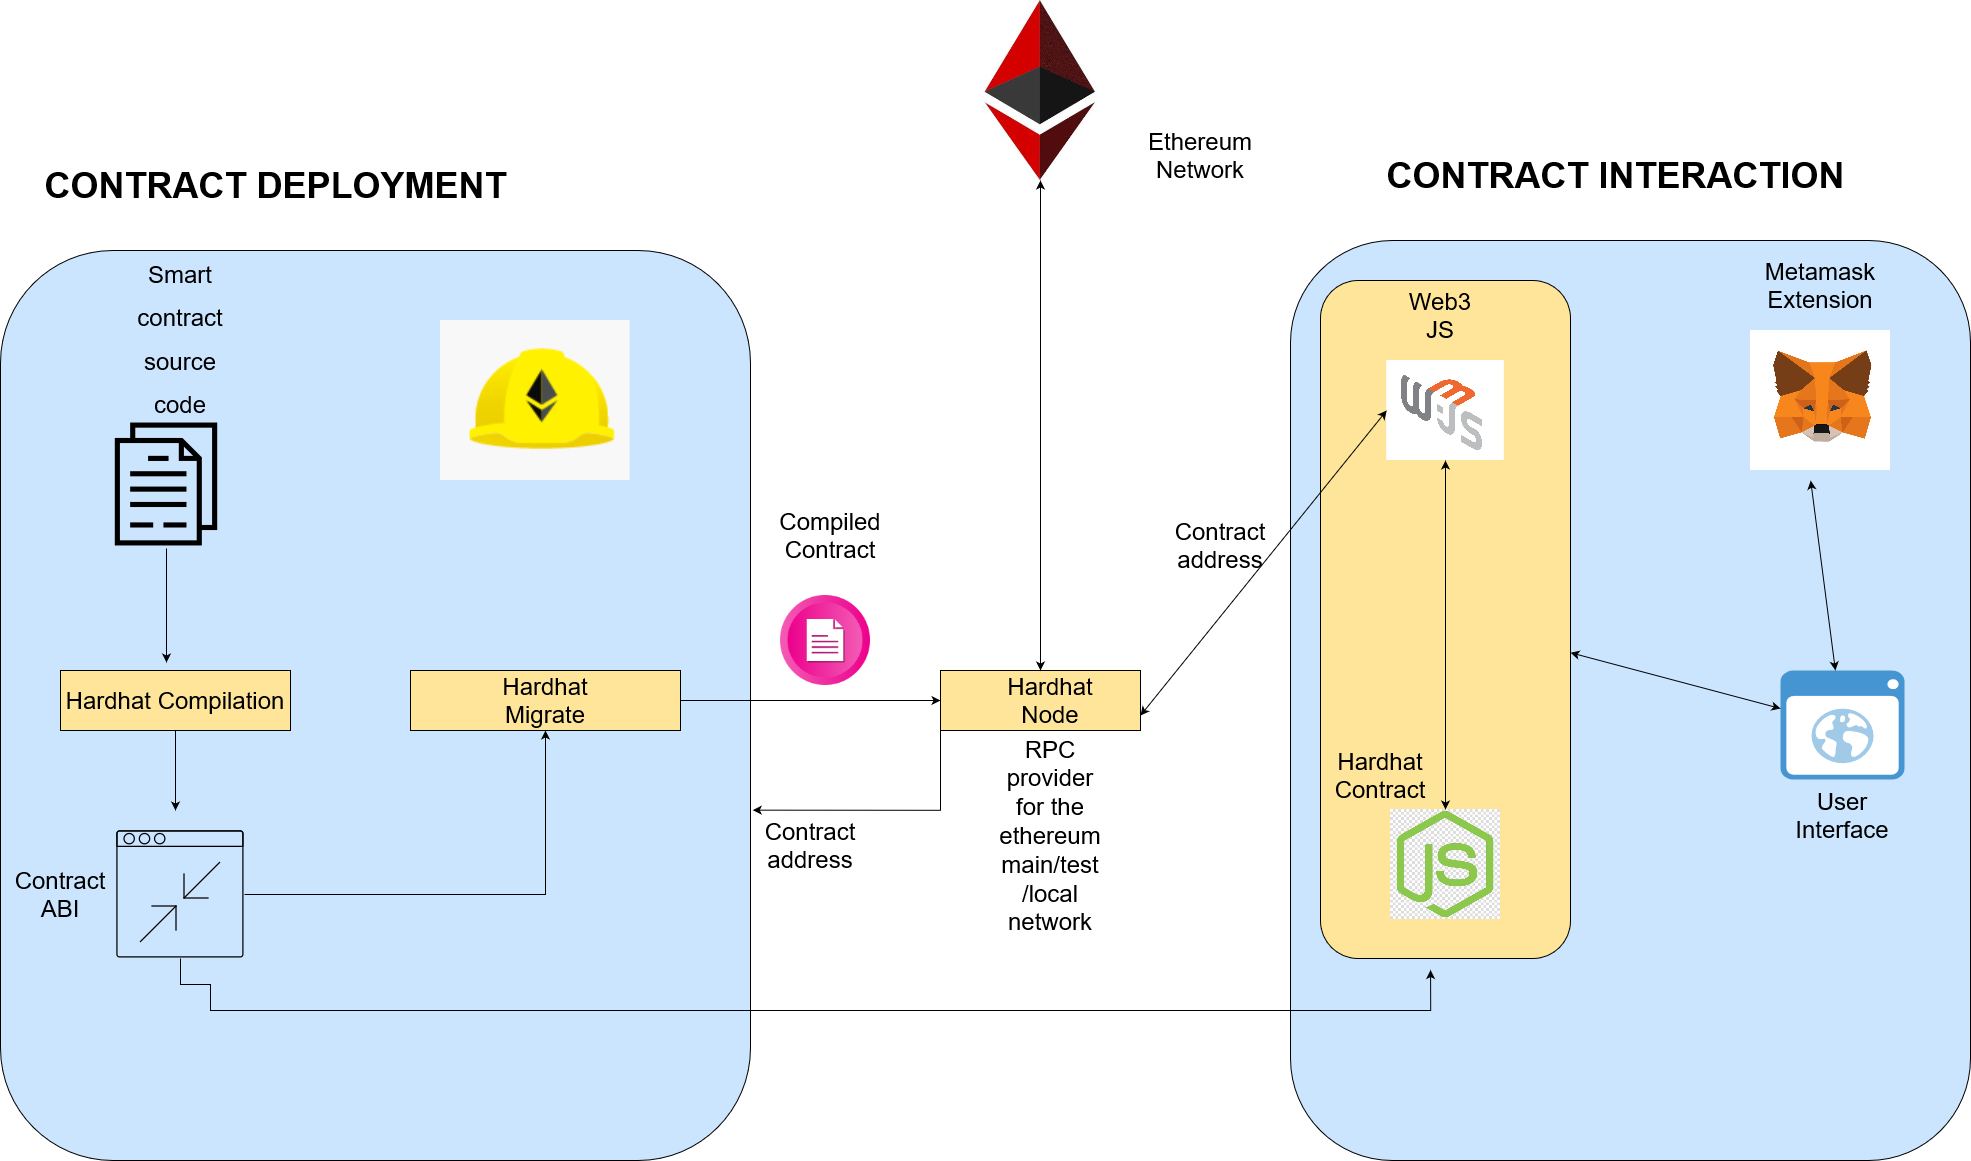
\includegraphics[width=\textwidth]{Untitled Diagram.drawio(1)}
\caption{Experimental Setup}
\end{figure}












\section{CONCLUSION}
The explosion in art based NFTs is a sign of a subtle paradigm shift in ways art is consumed. It directly affects both art and the artist. Working on and affecting key problems of the traditional setup such as accessibility to art, compensation of the artist, Ownership and licensing of media, the role of the middleman(art dealer) etc. It is with this in mind that we believe it worthwhile to pursue this project.\\
In this document, we have tried to provided a summarized, readable but also clear and informative sketch of the requirements of what our marketplace will be built on and what should be expected from the marketplace. We have tried to elucidate what blockchain is and how transactions work on it, what NFTs are and how they come into play in the world of digital collectibles, our  project methodologies, design ideas, development tools and also a risk-cost analysis which we think sufficiently covers the span of this project.In the next semester we will finalize the project and provide the marketplace to the jury, and then to the rest of the world in order for the marketplace to begin operation.\\
Our hope is to make a fully functional marketplace that will allow us to make a foray into this yet still emerging market that is showing so much promise as of now, NFTs can be used for not only  digital collectible media but also fund loaning systems, real estate,logistics, gaming and a whole host of other yet undiscovered pastures. The blockchain ledger is sure to be at the center of all things record keeping and transactions in the future to come.  














%
%% BIBLIOGRAPHY
%
\clearpage
\bibliographystyle{ieeetr}

\bibliography{sample}
\addcontentsline{toc}{section}{References}
\begin{flushleft}
\text{[1]} \url{https://www.npmjs.com/} 

\text{[2]} \url{https://docs.npmjs.com/cli/v6/commands/npm} 

\text{[3]} \url{https://www.ibm.com/topics/what-is-blockchain} 

\text{[4]} \url{https://www.nbcnews.com/tech/tech-news/nft-boom-digital-collectibles-rcna430} 

\text{[5]} \url{ https://www.securities.io/non-fungible-tokens-nfts-continue-to-reshape-the-blockchain-market/} 

\text{[6]} \url{https://pagepro.co/blog/what-is-nextjs/}

\text{[7]} \url{http://satoshinakamoto.me/bitcoin.pdf} 

\text{[8]} \url{https://hardhat.org/getting-started/} 

\text{[9]} \url{ https://infura.io/docs/ipfs} 

\end{flushleft}


%% USING .bib FILE
%


%
%% CREATING OWN BIBLIOGRAPHY
%

% \begin{thebibliography}{100}
% \bibitem{turing2009}{Turing, Alan M. "Computing machinery and intelligence." Parsing the Turing Test. Springer, Dordrecht, 2009. 23-65.}
% \bibitem{einstein1905} Albert Einstein. \textit{Zur Elektrodynamik bewegter K{\"o}rper}. (German) [\textit{On the electrodynamics of moving bodies}]. Annalen der Physik, 322(10):891–921, 1905.
% \end{thebibliography}


\end{document}
